% Advanced Data Analytics 2025 - Wrap-Up Lecture
% Week 14: Course Summary and Outlook
% Duration: 120 minutes

\documentclass[aspectratio=169,11pt]{beamer}

% Theme and color scheme
\usetheme{Madrid}
\usecolortheme{whale}
\setbeamertemplate{navigation symbols}{}
\setbeamertemplate{footline}[frame number]

% Packages
\usepackage[utf8]{inputenc}
\usepackage[T1]{fontenc}
\usepackage{amsmath,amssymb,amsfonts}
\usepackage{bm}
\usepackage{graphicx}
\usepackage{tikz}
\usetikzlibrary{shapes,arrows,positioning,calc,fit,backgrounds}
\usepackage{booktabs}
\usepackage{hyperref}
\usepackage{multicol}
\usepackage{xcolor}

% Custom colors
\definecolor{hec-blue}{RGB}{0,51,102}
\definecolor{hec-gold}{RGB}{204,153,0}
\definecolor{lightblue}{RGB}{173,216,230}
\definecolor{darkgreen}{RGB}{0,100,0}
\definecolor{darkred}{RGB}{139,0,0}

% Set beamer colors
\setbeamercolor{title}{fg=white,bg=hec-blue}
\setbeamercolor{frametitle}{fg=white,bg=hec-blue}
\setbeamercolor{structure}{fg=hec-blue}
\setbeamercolor{block title}{bg=hec-blue,fg=white}
\setbeamercolor{block body}{bg=lightblue!20}

% Math commands
\newcommand{\x}{\mathbf{x}}
\newcommand{\w}{\mathbf{w}}
\newcommand{\y}{\mathbf{y}}
\newcommand{\X}{\mathbf{X}}
\newcommand{\R}{\mathbb{R}}
\newcommand{\E}[1]{\mathbb{E}\left[ #1 \right]}
\DeclareMathOperator*{\argmin}{arg\,min}
\DeclareMathOperator*{\argmax}{arg\,max}

% Title information
\title[ADA 2025 - Wrap-Up]{Advanced Data Analytics 2025\\[0.5em]\large Course Wrap-Up and Outlook}
\author{Simon Scheidegger}
\institute{HEC Lausanne, University of Lausanne}
\date{Week 14 -- Monday, December 15, 2025}

\begin{document}

% =============================================================================
% TITLE SLIDE
% =============================================================================
\begin{frame}
\titlepage
\end{frame}

% =============================================================================
% OUTLINE
% =============================================================================
\begin{frame}{Today's Agenda (120 minutes)}
\begin{columns}
\column{0.5\textwidth}
\textbf{Part I: The Journey (40 min)}
\begin{itemize}
    \item From Newbie to AI Pioneer
    \item Course roadmap review
    \item The Machine Learning landscape
\end{itemize}

\vspace{1em}
\textbf{Part II: Core Concepts (40 min)}
\begin{itemize}
    \item Supervised Learning recap
    \item Deep Learning highlights
    \item Probabilistic methods
    \item Unsupervised \& RL
\end{itemize}

\column{0.5\textwidth}
\textbf{Part III: Integration (20 min)}
\begin{itemize}
    \item Connecting the dots
    \item Cross-cutting themes
    \item Method selection guide
\end{itemize}

\vspace{1em}
\textbf{Part IV: Looking Ahead (20 min)}
\begin{itemize}
    \item Current trends in ML/AI
    \item Career paths
    \item Capstone project advice
    \item Final thoughts
\end{itemize}
\end{columns}
\end{frame}

% =============================================================================
% PART I: THE JOURNEY
% =============================================================================
\section{Part I: The Journey}

\begin{frame}{}
\begin{center}
{\Huge \textcolor{hec-blue}{Part I}}\\[1em]
{\LARGE The Journey: From Newbie to AI Pioneer}
\end{center}
\end{frame}

\begin{frame}{Your Transformation Over 14 Weeks}
\begin{columns}
\column{0.33\textwidth}
\begin{center}
\textbf{Weeks 1-3}\\
\textit{The Newbie}\\[0.5em]
\includegraphics[width=0.9\textwidth]{../../../fig/fig1.png}\\[0.5em]
{\small Python? NumPy? Help!}
\end{center}

\column{0.33\textwidth}
\begin{center}
\textbf{Weeks 4-12}\\
\textit{The Learner}\\[0.5em]
\includegraphics[width=0.9\textwidth]{../../../fig/fig2.png}\\[0.5em]
{\small Neural networks, GPs, Clustering...}
\end{center}

\column{0.33\textwidth}
\begin{center}
\textbf{Week 14+}\\
\textit{The AI Pioneer}\\[0.5em]
\includegraphics[width=0.9\textwidth]{../../../fig/fig3.png}\\[0.5em]
{\small Ready to tackle real problems!}
\end{center}
\end{columns}
\end{frame}

\begin{frame}{The Course Roadmap}
\begin{center}
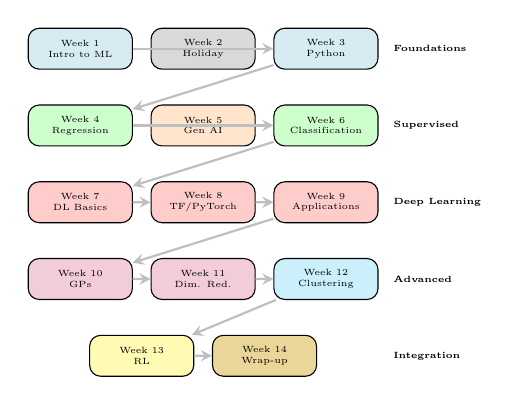
\begin{tikzpicture}[scale=0.65, transform shape,
    block/.style={rectangle, draw, fill=hec-blue!20, text width=1.8cm, text centered, rounded corners, minimum height=0.8cm, font=\tiny},
    arrow/.style={->, thick, >=stealth}]

    % Row 1: Foundations
    \node[block, fill=lightblue!50] (w1) at (0,0) {Week 1\\Intro to ML};
    \node[block, fill=gray!30] (w2) at (2.4,0) {Week 2\\Holiday};
    \node[block, fill=lightblue!50] (w3) at (4.8,0) {Week 3\\Python};

    % Row 2: Supervised Learning
    \node[block, fill=green!20] (w4) at (0,-1.5) {Week 4\\Regression};
    \node[block, fill=orange!20] (w5) at (2.4,-1.5) {Week 5\\Gen AI};
    \node[block, fill=green!20] (w6) at (4.8,-1.5) {Week 6\\Classification};

    % Row 3: Deep Learning
    \node[block, fill=red!20] (w7) at (0,-3) {Week 7\\DL Basics};
    \node[block, fill=red!20] (w8) at (2.4,-3) {Week 8\\TF/PyTorch};
    \node[block, fill=red!20] (w9) at (4.8,-3) {Week 9\\Applications};

    % Row 4: Advanced Methods
    \node[block, fill=purple!20] (w10) at (0,-4.5) {Week 10\\GPs};
    \node[block, fill=purple!20] (w11) at (2.4,-4.5) {Week 11\\Dim. Red.};
    \node[block, fill=cyan!20] (w12) at (4.8,-4.5) {Week 12\\Clustering};

    % Row 5: RL and Wrap-up
    \node[block, fill=yellow!30] (w13) at (1.2,-6) {Week 13\\RL};
    \node[block, fill=hec-gold!40] (w14) at (3.6,-6) {Week 14\\Wrap-up};

    % Labels
    \node[right, font=\tiny] at (6,0) {\textbf{Foundations}};
    \node[right, font=\tiny] at (6,-1.5) {\textbf{Supervised}};
    \node[right, font=\tiny] at (6,-3) {\textbf{Deep Learning}};
    \node[right, font=\tiny] at (6,-4.5) {\textbf{Advanced}};
    \node[right, font=\tiny] at (6,-6) {\textbf{Integration}};

    % Arrows showing progression
    \draw[arrow, gray!50] (w1) -- (w3);
    \draw[arrow, gray!50] (w3) -- (w4);
    \draw[arrow, gray!50] (w4) -- (w6);
    \draw[arrow, gray!50] (w6) -- (w7);
    \draw[arrow, gray!50] (w7) -- (w8);
    \draw[arrow, gray!50] (w8) -- (w9);
    \draw[arrow, gray!50] (w9) -- (w10);
    \draw[arrow, gray!50] (w10) -- (w11);
    \draw[arrow, gray!50] (w11) -- (w12);
    \draw[arrow, gray!50] (w12) -- (w13);
    \draw[arrow, gray!50] (w13) -- (w14);
\end{tikzpicture}
\end{center}
\end{frame}

\begin{frame}{The Machine Learning Landscape}
\begin{center}
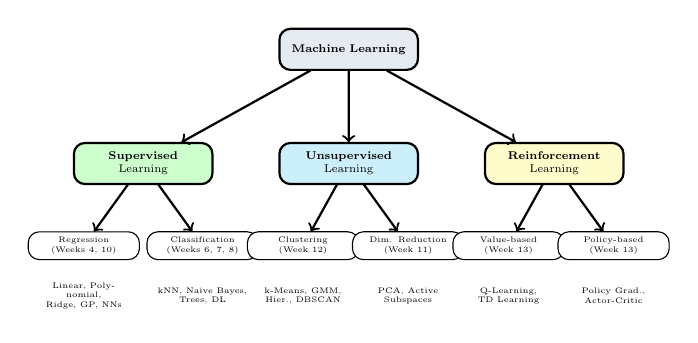
\begin{tikzpicture}[scale=0.58, transform shape,
    mainbox/.style={rectangle, draw, thick, fill=hec-blue!10, text width=2.8cm, text centered, rounded corners, minimum height=0.9cm, font=\scriptsize},
    subbox/.style={rectangle, draw, fill=white, text width=2.2cm, text centered, rounded corners, font=\tiny, minimum height=0.6cm}]

    % Main categories
    \node[mainbox] (ml) at (0,2.5) {\textbf{Machine Learning}};

    \node[mainbox, fill=green!20] (sup) at (-4.5,0) {\textbf{Supervised}\\Learning};
    \node[mainbox, fill=cyan!20] (unsup) at (0,0) {\textbf{Unsupervised}\\Learning};
    \node[mainbox, fill=yellow!20] (rl) at (4.5,0) {\textbf{Reinforcement}\\Learning};

    % Supervised subcategories
    \node[subbox] (reg) at (-5.8,-1.8) {Regression\\(Weeks 4, 10)};
    \node[subbox] (cls) at (-3.2,-1.8) {Classification\\(Weeks 6, 7, 8)};

    % Unsupervised subcategories
    \node[subbox] (clust) at (-1,-1.8) {Clustering\\(Week 12)};
    \node[subbox] (dim) at (1.3,-1.8) {Dim. Reduction\\(Week 11)};

    % RL subcategories
    \node[subbox] (val) at (3.5,-1.8) {Value-based\\(Week 13)};
    \node[subbox] (pol) at (5.8,-1.8) {Policy-based\\(Week 13)};

    % Methods under each
    \node[font=\tiny, text width=2cm, align=center] at (-5.8,-2.9) {Linear, Polynomial,\\Ridge, GP, NNs};
    \node[font=\tiny, text width=2cm, align=center] at (-3.2,-2.9) {kNN, Naive Bayes,\\Trees, DL};
    \node[font=\tiny, text width=2cm, align=center] at (-1,-2.9) {k-Means, GMM,\\Hier., DBSCAN};
    \node[font=\tiny, text width=2cm, align=center] at (1.3,-2.9) {PCA, Active\\Subspaces};
    \node[font=\tiny, text width=2cm, align=center] at (3.5,-2.9) {Q-Learning,\\TD Learning};
    \node[font=\tiny, text width=2cm, align=center] at (5.8,-2.9) {Policy Grad.,\\Actor-Critic};

    % Arrows
    \draw[->, thick] (ml) -- (sup);
    \draw[->, thick] (ml) -- (unsup);
    \draw[->, thick] (ml) -- (rl);
    \draw[->, thick] (sup) -- (reg);
    \draw[->, thick] (sup) -- (cls);
    \draw[->, thick] (unsup) -- (clust);
    \draw[->, thick] (unsup) -- (dim);
    \draw[->, thick] (rl) -- (val);
    \draw[->, thick] (rl) -- (pol);
\end{tikzpicture}
\end{center}
\end{frame}

\begin{frame}{What You've Learned: By the Numbers}
\begin{columns}
\column{0.5\textwidth}
\begin{block}{Methods Covered}
\begin{itemize}
    \item \textbf{7+} regression techniques
    \item \textbf{5+} classification algorithms
    \item \textbf{4} clustering methods
    \item \textbf{3} dimensionality reduction approaches
    \item \textbf{2} reinforcement learning paradigms
\end{itemize}
\end{block}

\column{0.5\textwidth}
\begin{block}{Tools \& Frameworks}
\begin{itemize}
    \item \textbf{Python} ecosystem
    \item \textbf{NumPy, SciPy, Pandas}
    \item \textbf{scikit-learn}
    \item \textbf{TensorFlow \& PyTorch}
    \item \textbf{GPFlow}
    \item \textbf{Jupyter Notebooks}
\end{itemize}
\end{block}
\end{columns}

\vspace{1em}
\begin{block}{Application Domains}
Finance (option pricing, portfolio optimization), Economics (dynamic models), Climate science, Natural language processing, Computer vision, Time series forecasting
\end{block}
\end{frame}

% =============================================================================
% PART II: CORE CONCEPTS
% =============================================================================
\section{Part II: Core Concepts Recap}

\begin{frame}{}
\begin{center}
{\Huge \textcolor{hec-blue}{Part II}}\\[1em]
{\LARGE Core Concepts Recap}
\end{center}
\end{frame}

% -----------------------------------------------------------------------------
% SUPERVISED LEARNING
% -----------------------------------------------------------------------------
\subsection{Supervised Learning}

\begin{frame}{Supervised Learning: The Big Picture}
\begin{block}{The Setup}
Given training data $\mathcal{D} = \{(\x_i, y_i)\}_{i=1}^N$, learn a function $f: \mathcal{X} \to \mathcal{Y}$
\end{block}

\begin{columns}
\column{0.5\textwidth}
\textbf{Regression} ($y \in \R$)
\begin{itemize}
    \item Linear: $f(\x) = \w^\top \x$
    \item Polynomial: $f(\x) = \sum_j w_j \phi_j(\x)$
    \item Neural Networks: $f = f_L \circ \cdots \circ f_1$
    \item Gaussian Processes
\end{itemize}

\column{0.5\textwidth}
\textbf{Classification} ($y \in \{0,1,\ldots,K\}$)
\begin{itemize}
    \item k-Nearest Neighbors
    \item Naive Bayes
    \item Decision Trees
    \item Neural Networks (softmax)
\end{itemize}
\end{columns}

\vspace{0.5em}
\begin{alertblock}{Key Principle}
\textbf{Minimize empirical risk} while \textbf{controlling model complexity}
\end{alertblock}
\end{frame}

\begin{frame}{The Bias-Variance Tradeoff}
\begin{columns}
\column{0.52\textwidth}
\begin{block}{Expected Error Decomposition}
{\small
\[
\E{(y - \hat{f})^2} = \text{Bias}^2 + \text{Var} + \sigma^2
\]
}
\end{block}

\begin{itemize}
    \item \textbf{High Bias}: Too simple $\to$ \textcolor{darkred}{Underfitting}
    \item \textbf{High Variance}: Too complex $\to$ \textcolor{darkred}{Overfitting}
    \item \textbf{Goal}: Find the sweet spot!
\end{itemize}

\column{0.48\textwidth}
\begin{center}
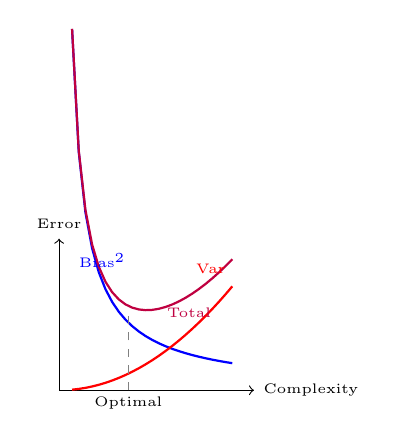
\begin{tikzpicture}[scale=0.55]
    \draw[->] (0,0) -- (4.5,0) node[right] {\tiny Complexity};
    \draw[->] (0,0) -- (0,3.5) node[above] {\tiny Error};

    % Bias curve (decreasing)
    \draw[thick, blue, domain=0.3:4] plot (\x, {2.5/\x});

    % Variance curve (increasing)
    \draw[thick, red, domain=0.3:4] plot (\x, {0.15*\x*\x});

    % Total error
    \draw[thick, purple, domain=0.3:4] plot (\x, {2.5/\x + 0.15*\x*\x});

    % Labels
    \node[blue, font=\tiny] at (1,3) {Bias$^2$};
    \node[red, font=\tiny] at (3.5,2.8) {Var};
    \node[purple, font=\tiny] at (3,1.8) {Total};

    % Optimal point
    \draw[dashed, gray] (1.6,0) -- (1.6,1.9);
    \node[font=\tiny] at (1.6,-0.3) {Optimal};
\end{tikzpicture}
\end{center}
\end{columns}

\vspace{0.3em}
{\small \textbf{Strategies}: Regularization, Cross-validation, Early stopping, Dropout, Ensembles}
\end{frame}

\begin{frame}{Gradient Descent: The Workhorse of ML}
\begin{columns}
\column{0.55\textwidth}
\begin{block}{The Algorithm}
\textbf{Goal}: Minimize loss $\mathcal{L}(\bm{\theta})$
\[
\bm{\theta}^{(t+1)} = \bm{\theta}^{(t)} - \alpha \nabla_{\bm{\theta}} \mathcal{L}(\bm{\theta}^{(t)})
\]
\end{block}

\textbf{Variants covered}:
\begin{itemize}
    \item \textbf{Batch GD}: Use all data each step
    \item \textbf{Stochastic GD}: Use one sample
    \item \textbf{Mini-batch GD}: Use small batches
    \item \textbf{Adam, RMSprop}: Adaptive learning rates
\end{itemize}

\column{0.45\textwidth}
\begin{center}
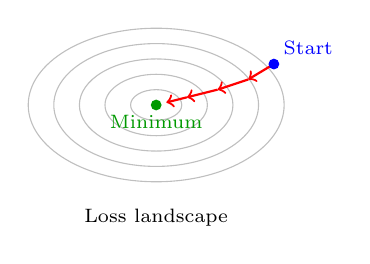
\begin{tikzpicture}[scale=0.65]
    % Contour lines
    \foreach \r in {0.5, 1, 1.5, 2, 2.5} {
        \draw[gray!50] (0,0) ellipse ({\r} and {0.6*\r});
    }

    % Gradient descent path
    \draw[thick, red, ->] (2.3, 0.8) -- (1.8, 0.5);
    \draw[thick, red, ->] (1.8, 0.5) -- (1.2, 0.3);
    \draw[thick, red, ->] (1.2, 0.3) -- (0.6, 0.15);
    \draw[thick, red, ->] (0.6, 0.15) -- (0.2, 0.05);

    % Start and end points
    \fill[blue] (2.3, 0.8) circle (3pt) node[above right, font=\scriptsize] {Start};
    \fill[green!60!black] (0,0) circle (3pt) node[below, font=\scriptsize] {Minimum};

    \node[font=\scriptsize] at (0, -2.2) {Loss landscape};
\end{tikzpicture}
\end{center}
\end{columns}

\vspace{0.5em}
\begin{alertblock}{Key Insight}
SGD's noise actually helps escape local minima -- crucial for deep learning!
\end{alertblock}
\end{frame}

\begin{frame}{Linear Regression to Neural Networks: A Continuum}
\begin{center}
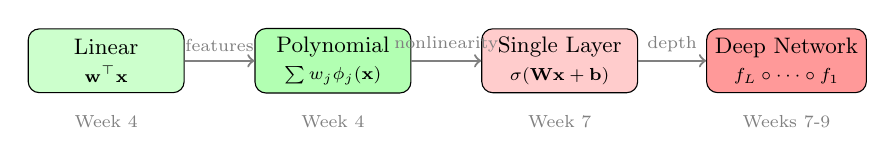
\begin{tikzpicture}[scale=0.9, transform shape,
    box/.style={rectangle, draw, fill=white, minimum width=2.2cm, minimum height=0.9cm, font=\small, align=center, rounded corners}]

    % Linear
    \node[box, fill=green!20] (lin) at (0,0) {Linear\\{\scriptsize $\w^\top\x$}};

    % Polynomial
    \node[box, fill=green!30] (poly) at (3.2,0) {Polynomial\\{\scriptsize $\sum w_j\phi_j(\x)$}};

    % Single layer
    \node[box, fill=red!20] (sl) at (6.4,0) {Single Layer\\{\scriptsize $\sigma(\mathbf{W}\x + \mathbf{b})$}};

    % Deep
    \node[box, fill=red!40] (deep) at (9.6,0) {Deep Network\\{\scriptsize $f_L \circ \cdots \circ f_1$}};

    % Arrows with labels
    \draw[->, thick, gray] (lin) -- (poly) node[midway, above, font=\scriptsize] {features};
    \draw[->, thick, gray] (poly) -- (sl) node[midway, above, font=\scriptsize] {nonlinearity};
    \draw[->, thick, gray] (sl) -- (deep) node[midway, above, font=\scriptsize] {depth};

    % Week annotations below
    \node[font=\scriptsize, gray] at (0,-0.85) {Week 4};
    \node[font=\scriptsize, gray] at (3.2,-0.85) {Week 4};
    \node[font=\scriptsize, gray] at (6.4,-0.85) {Week 7};
    \node[font=\scriptsize, gray] at (9.6,-0.85) {Weeks 7-9};
\end{tikzpicture}
\end{center}

\vspace{0.3em}
\begin{columns}
\column{0.5\textwidth}
{\small \textbf{Common thread}: Minimize a loss function}
{\small \[\mathcal{L}(\bm{\theta}) = \frac{1}{N}\sum_{i=1}^N \ell(y_i, f(\x_i; \bm{\theta}))\]}

\column{0.5\textwidth}
{\small \textbf{Regularization throughout}:}
\begin{itemize}
    \item Ridge/Lasso for linear models
    \item Weight decay for neural networks
    \item Dropout, batch normalization
\end{itemize}
\end{columns}
\end{frame}

\begin{frame}{Classification: From Simple to Sophisticated}
\begin{columns}
\column{0.5\textwidth}
\textbf{k-Nearest Neighbors}
\begin{itemize}
    \item Non-parametric, instance-based
    \item Prediction: majority vote of k nearest
    \item Key: choice of k and distance metric
\end{itemize}

\vspace{0.5em}
\textbf{Naive Bayes}
\begin{itemize}
    \item Probabilistic: $P(y|\x) \propto P(y)\prod_j P(x_j|y)$
    \item ``Naive'' independence assumption
    \item Fast, works well for text
\end{itemize}

\column{0.5\textwidth}
\textbf{Decision Trees}
\begin{itemize}
    \item Interpretable, hierarchical rules
    \item Split on features to maximize info gain
    \item Prone to overfitting $\to$ pruning
\end{itemize}

\vspace{0.5em}
\textbf{Ensemble Methods}
\begin{itemize}
    \item \textbf{Bagging}: Average many trees (Random Forest)
    \item \textbf{Boosting}: Sequentially fix errors
    \item Often best ``out of the box'' performance
\end{itemize}
\end{columns}

\vspace{0.5em}
\begin{block}{Evaluation Metrics}
Accuracy, Precision, Recall, F1-score, ROC-AUC, Confusion Matrix
\end{block}
\end{frame}

% -----------------------------------------------------------------------------
% DEEP LEARNING
% -----------------------------------------------------------------------------
\subsection{Deep Learning}

\begin{frame}{Deep Learning: Key Architectures}
\begin{columns}
\column{0.5\textwidth}
\textbf{Feed-Forward Networks (FFN)}
\begin{itemize}
    \item Layers: Input $\to$ Hidden $\to$ Output
    \item Universal approximation theorem
    \item Applications: tabular data, function approximation
\end{itemize}

\vspace{0.5em}
\textbf{Recurrent Neural Networks (RNN)}
\begin{itemize}
    \item Sequential data processing
    \item Hidden state carries information
    \item Challenge: vanishing gradients
\end{itemize}

\column{0.5\textwidth}
\textbf{Long Short-Term Memory (LSTM)}
\begin{itemize}
    \item Gates: forget, input, output
    \item Cell state for long-term memory
    \item Applications: time series, NLP
\end{itemize}

\vspace{0.5em}
\textbf{Transformers} (Glimpse)
\begin{itemize}
    \item Self-attention mechanism
    \item Parallel processing
    \item Foundation for LLMs (GPT, etc.)
\end{itemize}
\end{columns}
\end{frame}

\begin{frame}{LSTM: The Gates that Remember}
\begin{columns}
\column{0.52\textwidth}
{\small \textbf{Three Gates + Cell State}:}
\begin{enumerate}
    \item \textbf{Forget}: $f_t = \sigma(W_f[h_{t-1}, x_t] + b_f)$
    \item \textbf{Input}: $i_t = \sigma(W_i[h_{t-1}, x_t] + b_i)$
    \item \textbf{Output}: $o_t = \sigma(W_o[h_{t-1}, x_t] + b_o)$
\end{enumerate}

{\small \textbf{Cell State}: $C_t = f_t \odot C_{t-1} + i_t \odot \tilde{C}_t$}

\column{0.48\textwidth}
\begin{center}

\includegraphics[width=0.95\textwidth]{../../lecture_9/demo/figures/LSTM3-chain.png}
\end{center}
{\tiny \textit{Source: C. Olah's blog}}
\end{columns}

\vspace{0.2em}
{\small \textbf{Applications}: Stock prices, weather, time series}
\end{frame}

\begin{frame}{TensorFlow vs PyTorch: Your Deep Learning Toolbox}
\begin{columns}
\column{0.5\textwidth}
\begin{block}{TensorFlow}
\begin{itemize}
    \item Production-ready, scalable
    \item TensorBoard for visualization
    \item Keras API for ease of use
    \item Static graph (eager mode available)
    \item Strong deployment ecosystem
\end{itemize}
\end{block}

\column{0.5\textwidth}
\begin{block}{PyTorch}
\begin{itemize}
    \item Research-friendly, Pythonic
    \item Dynamic computation graph
    \item Easy debugging
    \item Strong in academia
    \item torchvision, torchaudio, etc.
\end{itemize}
\end{block}
\end{columns}

\vspace{1em}
\begin{alertblock}{Practical Advice}
\begin{itemize}
    \item Both are excellent choices -- pick based on your use case
    \item For research/prototyping: PyTorch often preferred
    \item For production/deployment: TensorFlow has mature tools
    \item Learn one well, the concepts transfer!
\end{itemize}
\end{alertblock}
\end{frame}

\begin{frame}{Neural Networks for Economics \& Finance}
\textbf{Applications covered in Weeks 9 \& 14:}

\begin{columns}
\column{0.5\textwidth}
\begin{block}{Physics-Informed NNs (PINNs)}
\begin{itemize}
    \item Embed PDEs as constraints
    \item Option pricing (Black-Scholes)
    \item Respects domain knowledge
\end{itemize}
\end{block}

\begin{block}{Deep Equilibrium Networks}
\begin{itemize}
    \item Solve dynamic economic models
    \item Handle high-dimensional states
    \item Uncertainty quantification
\end{itemize}
\end{block}

\column{0.5\textwidth}
\begin{block}{Key Insight}
Neural networks as \textbf{function approximators} for:
\begin{itemize}
    \item Value functions
    \item Policy functions
    \item Pricing functions
    \item Equilibrium mappings
\end{itemize}
\end{block}

\vspace{0.5em}
\textbf{Why it works}:
\begin{itemize}
    \item Universal approximation
    \item Handles curse of dimensionality
    \item GPU acceleration
\end{itemize}
\end{columns}
\end{frame}

% -----------------------------------------------------------------------------
% PROBABILISTIC METHODS
% -----------------------------------------------------------------------------
\subsection{Probabilistic Methods}

\begin{frame}{Gaussian Processes: Bayesian Non-parametric Regression}
\begin{columns}
\column{0.52\textwidth}
\begin{block}{Key Idea}
Prior over \textbf{functions}: $f(\x) \sim \mathcal{GP}(m(\x), k(\x, \x'))$
\end{block}

{\small \textbf{Components}:}
\begin{itemize}
    \item Mean function $m(\x)$
    \item Kernel $k(\x, \x')$ (RBF, Matérn)
\end{itemize}

{\small \textbf{Posterior}: $f_* | \X, \y \sim \mathcal{N}(\mu_*, \Sigma_*)$}

\column{0.48\textwidth}
\begin{center}

\includegraphics[width=0.9\textwidth]{../../lecture_10/demo_GP/draw_prediction.png}
\end{center}
{\tiny GP prediction with uncertainty}
\end{columns}

\vspace{0.2em}
\begin{alertblock}{Why GPs Matter}
\textbf{Built-in uncertainty quantification!} Know what you don't know.
\end{alertblock}
\end{frame}

\begin{frame}{The Curse of Dimensionality \& Solutions}
\begin{columns}
\column{0.5\textwidth}
\begin{block}{The Problem}
As dimension $d$ increases:
\begin{itemize}
    \item Data becomes sparse
    \item Distance metrics lose meaning
    \item Sample complexity explodes
    \item $N \sim O(\epsilon^{-d})$ for $\epsilon$-covering
\end{itemize}
\end{block}

\column{0.5\textwidth}
\begin{block}{Solutions (Week 11)}
\begin{itemize}
    \item \textbf{PCA}: Linear projection to lower-D
    \item \textbf{Active Subspaces}: Find important directions
    \item \textbf{Deep Kernel Learning}: Non-linear dim. reduction + GP
    \item \textbf{Active Learning}: Query where it matters
\end{itemize}
\end{block}
\end{columns}

\vspace{0.5em}
\textbf{Principal Component Analysis}:
\begin{itemize}
    \item Find orthogonal directions of maximum variance
    \item Project data: $\mathbf{z} = \mathbf{W}^\top (\x - \bm{\mu})$
    \item Keep top $k$ components explaining most variance
\end{itemize}
\end{frame}

\begin{frame}{Bayesian Active Learning}
\begin{columns}
\column{0.55\textwidth}
\begin{block}{The Idea}
Sample where \textbf{uncertainty is highest}!
\end{block}

{\small \textbf{Acquisition Functions}:}
\begin{itemize}
    \item \textbf{Uncertainty}: $\x^* = \argmax_\x \sigma(\x)$
    \item \textbf{Expected Improvement}
    \item \textbf{Information Gain}
\end{itemize}

{\small \textbf{Benefits}: Fewer samples, targeted exploration}

\column{0.45\textwidth}
\begin{center}
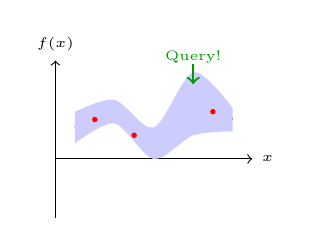
\begin{tikzpicture}[scale=0.5]
    \draw[->] (0,0) -- (5,0) node[right] {\tiny $x$};
    \draw[->] (0,-1.5) -- (0,2.5) node[above] {\tiny $f(x)$};

    % Mean prediction
    \draw[thick, blue, smooth] plot coordinates {(0.5,0.8) (1.5,1.2) (2.5,0.4) (3.5,1.4) (4.5,1)};

    % Uncertainty band
    \fill[blue!20, smooth] plot coordinates {(0.5,0.4) (1.5,0.9) (2.5,0) (3.5,0.6) (4.5,0.7)}
    -- plot coordinates {(4.5,1.3) (3.5,2.2) (2.5,0.8) (1.5,1.5) (0.5,1.2)} -- cycle;

    % Data points
    \fill[red] (1,1) circle (2pt);
    \fill[red] (2,0.6) circle (2pt);
    \fill[red] (4,1.2) circle (2pt);

    % Next query point
    \draw[thick, green!60!black, ->] (3.5,2.4) -- (3.5,1.9);
    \node[font=\tiny, green!60!black] at (3.5,2.6) {Query!};
\end{tikzpicture}
\end{center}
\end{columns}
\end{frame}

% -----------------------------------------------------------------------------
% UNSUPERVISED & RL
% -----------------------------------------------------------------------------
\subsection{Unsupervised Learning \& RL}

\begin{frame}{Clustering: Finding Structure in Data}
\begin{columns}
\column{0.5\textwidth}
\textbf{k-Means}
\begin{itemize}
    \item Assign points to nearest centroid
    \item Update centroids iteratively
    \item Converges to local minimum
    \item Choose $k$ via elbow method, silhouette
\end{itemize}

\vspace{0.5em}
\textbf{Gaussian Mixture Models}
\begin{itemize}
    \item Soft clustering (probabilities)
    \item EM algorithm for fitting
    \item More flexible than k-means
\end{itemize}

\column{0.5\textwidth}
\textbf{Hierarchical Clustering}
\begin{itemize}
    \item Agglomerative (bottom-up)
    \item Divisive (top-down)
    \item Dendrogram visualization
    \item No need to specify $k$ upfront
\end{itemize}

\vspace{0.5em}
\textbf{DBSCAN}
\begin{itemize}
    \item Density-based
    \item Finds arbitrary shapes
    \item Handles noise/outliers
    \item Parameters: $\epsilon$, minPts
\end{itemize}
\end{columns}
\end{frame}

\begin{frame}{Reinforcement Learning: Learning from Interaction}
\begin{columns}
\column{0.5\textwidth}
\begin{block}{The Setup}
{\small Agent interacts with environment:}
\begin{itemize}
    \item \textbf{State} $s_t$: Current situation
    \item \textbf{Action} $a_t$: Agent's choice
    \item \textbf{Reward} $r_t$: Feedback signal
    \item \textbf{Policy} $\pi(a|s)$: Decision rule
\end{itemize}
\end{block}

\column{0.5\textwidth}
\begin{center}
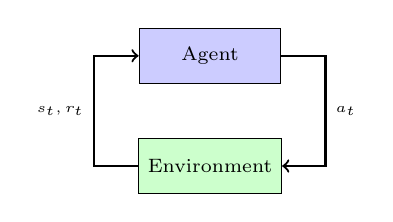
\begin{tikzpicture}[scale=0.7,
    box/.style={rectangle, draw, minimum width=1.8cm, minimum height=0.7cm, font=\scriptsize}]

    \node[box, fill=blue!20] (agent) at (0,1.2) {Agent};
    \node[box, fill=green!20] (env) at (0,-0.8) {Environment};

    \draw[->, thick] (agent.east) -- ++(0.8,0) |- node[right, pos=0.25, font=\tiny] {$a_t$} (env.east);
    \draw[->, thick] (env.west) -- ++(-0.8,0) |- node[left, pos=0.25, font=\tiny] {$s_t, r_t$} (agent.west);
\end{tikzpicture}
\end{center}
\end{columns}

\vspace{0.3em}
{\small \textbf{Goal}: Maximize $V^\pi(s) = \E{\sum_{t=0}^\infty \gamma^t r_t | s_0 = s}$}

\vspace{0.2em}
{\small \textbf{Q-Learning}: $Q(s,a) \leftarrow Q(s,a) + \alpha[r + \gamma \max_{a'} Q(s',a') - Q(s,a)]$}
\end{frame}

\begin{frame}{RL Application: Portfolio Optimization}
\begin{columns}
\column{0.55\textwidth}
\textbf{Problem Formulation}:
\begin{itemize}
    \item \textbf{State}: Portfolio weights, market conditions
    \item \textbf{Action}: Rebalancing decisions
    \item \textbf{Reward}: Risk-adjusted returns
\end{itemize}

\vspace{0.5em}
\textbf{Why RL for Finance?}
\begin{itemize}
    \item Sequential decision problem
    \item Non-stationary markets
    \item Complex constraints
    \item Transaction costs matter
\end{itemize}

\column{0.45\textwidth}
\begin{block}{Markowitz meets RL}
\begin{itemize}
    \item Classic: One-period optimization
    \item RL: Multi-period, dynamic
    \item Learn optimal policy over time
    \item Handle realistic constraints
\end{itemize}
\end{block}
\end{columns}

\vspace{0.5em}
\begin{alertblock}{Covered in Week 13}
Least-squares policy iteration for portfolio choice with realistic market dynamics
\end{alertblock}
\end{frame}

% =============================================================================
% PART III: INTEGRATION
% =============================================================================
\section{Part III: Connecting the Dots}

\begin{frame}{}
\begin{center}
{\Huge \textcolor{hec-blue}{Part III}}\\[1em]
{\LARGE Connecting the Dots}
\end{center}
\end{frame}

\begin{frame}{Cross-Cutting Themes}
\begin{columns}
\column{0.5\textwidth}
\begin{block}{1. Optimization Everywhere}
\begin{itemize}
    \item Linear regression $\to$ least squares
    \item Neural networks $\to$ SGD
    \item k-means $\to$ coordinate descent
    \item RL $\to$ policy optimization
\end{itemize}
\end{block}

\begin{block}{2. Regularization}
\begin{itemize}
    \item Ridge, Lasso (linear)
    \item Weight decay, dropout (DL)
    \item Kernel choice (GPs)
    \item Tree pruning (decision trees)
\end{itemize}
\end{block}

\column{0.5\textwidth}
\begin{block}{3. Probabilistic Thinking}
\begin{itemize}
    \item Naive Bayes
    \item Gaussian Processes
    \item Mixture Models
    \item Uncertainty quantification
\end{itemize}
\end{block}

\begin{block}{4. Feature Representation}
\begin{itemize}
    \item Feature engineering (manual)
    \item Kernel methods (implicit)
    \item Deep learning (learned)
    \item PCA (linear extraction)
\end{itemize}
\end{block}
\end{columns}
\end{frame}

\begin{frame}{Method Selection Guide}
\begin{center}
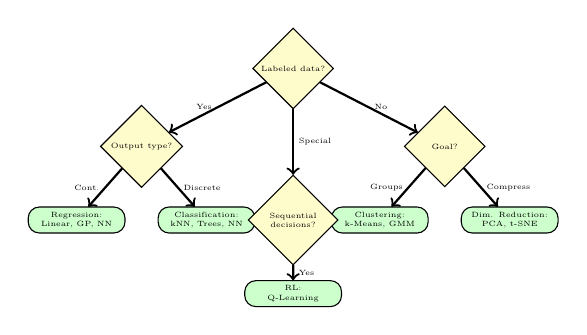
\begin{tikzpicture}[scale=0.55, transform shape,
    decision/.style={diamond, draw, fill=yellow!20, text width=1.6cm, text badly centered, inner sep=1pt, font=\tiny},
    block/.style={rectangle, draw, fill=green!20, text width=2cm, text centered, rounded corners, font=\tiny},
    arrow/.style={->, thick}]

    % Start
    \node[decision] (start) at (0,0) {Labeled data?};

    % Supervised branch
    \node[decision] (type) at (-3.5,-1.8) {Output type?};
    \node[block] (reg) at (-5,-3.5) {Regression:\\Linear, GP, NN};
    \node[block] (cls) at (-2,-3.5) {Classification:\\kNN, Trees, NN};

    % Unsupervised branch
    \node[decision] (goal) at (3.5,-1.8) {Goal?};
    \node[block] (clust) at (2,-3.5) {Clustering:\\k-Means, GMM};
    \node[block] (dim) at (5,-3.5) {Dim. Reduction:\\PCA, t-SNE};

    % RL branch
    \node[decision] (seq) at (0,-3.5) {Sequential\\decisions?};
    \node[block] (rl) at (0,-5.2) {RL:\\Q-Learning};

    % Arrows
    \draw[arrow] (start) -- node[left, font=\tiny] {Yes} (type);
    \draw[arrow] (start) -- node[right, font=\tiny] {No} (goal);
    \draw[arrow] (type) -- node[left, font=\tiny] {Cont.} (reg);
    \draw[arrow] (type) -- node[right, font=\tiny] {Discrete} (cls);
    \draw[arrow] (goal) -- node[left, font=\tiny] {Groups} (clust);
    \draw[arrow] (goal) -- node[right, font=\tiny] {Compress} (dim);
    \draw[arrow] (start) -- node[right, font=\tiny] {Special} (seq);
    \draw[arrow] (seq) -- node[right, font=\tiny] {Yes} (rl);
\end{tikzpicture}
\end{center}

\vspace{0.3em}
\textbf{Reality}: Often combine methods! GP + Deep Learning, Clustering + Classification, etc.
\end{frame}

\begin{frame}{The Data Science Workflow}
\begin{center}
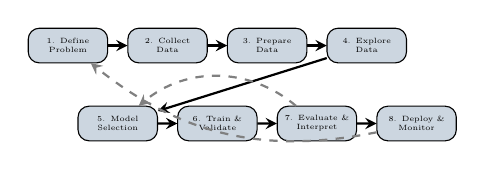
\begin{tikzpicture}[scale=0.55, transform shape,
    box/.style={rectangle, draw, fill=hec-blue!20, text width=1.6cm, text centered, rounded corners, minimum height=0.8cm, font=\tiny},
    arrow/.style={->, thick, >=stealth}]

    % Boxes - Row 1
    \node[box] (prob) at (0,0) {1. Define\\Problem};
    \node[box] (data) at (2.3,0) {2. Collect\\Data};
    \node[box] (prep) at (4.6,0) {3. Prepare\\Data};
    \node[box] (explore) at (6.9,0) {4. Explore\\Data};
    % Boxes - Row 2
    \node[box] (model) at (1.15,-1.8) {5. Model\\Selection};
    \node[box] (train) at (3.45,-1.8) {6. Train \&\\Validate};
    \node[box] (eval) at (5.75,-1.8) {7. Evaluate \&\\Interpret};
    \node[box] (deploy) at (8.05,-1.8) {8. Deploy \&\\Monitor};

    % Arrows
    \draw[arrow] (prob) -- (data);
    \draw[arrow] (data) -- (prep);
    \draw[arrow] (prep) -- (explore);
    \draw[arrow] (explore) -- (model);
    \draw[arrow] (model) -- (train);
    \draw[arrow] (train) -- (eval);
    \draw[arrow] (eval) -- (deploy);

    % Feedback loop
    \draw[arrow, dashed, gray] (eval) to[bend right=40] (model);
    \draw[arrow, dashed, gray] (deploy) to[bend left=25] (prob);
\end{tikzpicture}
\end{center}

\vspace{0.3em}
\begin{columns}
\column{0.5\textwidth}
\textbf{This course focused on}:
\begin{itemize}
    \item Steps 5-7 (modeling)
    \item Understanding algorithms
    \item Proper evaluation
\end{itemize}

\column{0.5\textwidth}
\textbf{In practice, also critical}:
\begin{itemize}
    \item Data quality \& preprocessing
    \item Feature engineering
    \item Deployment challenges
\end{itemize}
\end{columns}
\end{frame}

\begin{frame}{Common Pitfalls to Avoid}
\begin{columns}
\column{0.5\textwidth}
\begin{alertblock}{Data Leakage}
\begin{itemize}
    \item Using test data for training
    \item Feature engineering on full dataset
    \item \textbf{Solution}: Strict train/test split
\end{itemize}
\end{alertblock}

\begin{alertblock}{Overfitting}
\begin{itemize}
    \item Complex model, limited data
    \item Perfect training, poor test
    \item \textbf{Solution}: Regularization, cross-validation
\end{itemize}
\end{alertblock}

\column{0.5\textwidth}
\begin{alertblock}{Selection Bias}
\begin{itemize}
    \item Non-representative data
    \item Survivorship bias
    \item \textbf{Solution}: Careful data collection
\end{itemize}
\end{alertblock}

\begin{alertblock}{Ignoring Uncertainty}
\begin{itemize}
    \item Point predictions only
    \item Overconfident models
    \item \textbf{Solution}: Use GPs, ensembles, Bayesian methods
\end{itemize}
\end{alertblock}
\end{columns}
\end{frame}

% =============================================================================
% PART IV: LOOKING AHEAD
% =============================================================================
\section{Part IV: Looking Ahead}

\begin{frame}{}
\begin{center}
{\Huge \textcolor{hec-blue}{Part IV}}\\[1em]
{\LARGE Looking Ahead}
\end{center}
\end{frame}

\begin{frame}{Current Trends in ML/AI (2025)}
\begin{columns}
\column{0.5\textwidth}
\begin{block}{Large Language Models}
\begin{itemize}
    \item GPT-4, Claude, Llama, Gemini
    \item Transformers at scale
    \item Prompt engineering
    \item Multimodal capabilities
\end{itemize}
\end{block}

\begin{block}{Foundation Models}
\begin{itemize}
    \item Pre-train once, fine-tune many
    \item Transfer learning at scale
    \item Vision, language, multimodal
\end{itemize}
\end{block}

\column{0.5\textwidth}
\begin{block}{Scientific ML}
\begin{itemize}
    \item Physics-informed NNs
    \item Neural operators (PDEs)
    \item Drug discovery, materials
    \item Climate modeling
\end{itemize}
\end{block}

\begin{block}{Responsible AI}
\begin{itemize}
    \item Fairness \& bias mitigation
    \item Explainability (XAI)
    \item Privacy-preserving ML
    \item AI safety research
\end{itemize}
\end{block}
\end{columns}
\end{frame}

\begin{frame}{Career Paths in Data Science / ML}
\begin{columns}
\column{0.5\textwidth}
\begin{block}{Industry Roles}
\begin{itemize}
    \item \textbf{Data Scientist}: Analysis + ML
    \item \textbf{ML Engineer}: Production systems
    \item \textbf{Research Scientist}: New methods
    \item \textbf{Quant}: Finance + ML
    \item \textbf{AI Product Manager}: Strategy
\end{itemize}
\end{block}

\column{0.5\textwidth}
\begin{block}{Skill Development}
\begin{itemize}
    \item Deepen: Choose a specialization
    \item Broaden: Software engineering skills
    \item Practice: Kaggle, personal projects
    \item Network: Conferences, meetups
    \item Stay current: Papers, blogs, courses
\end{itemize}
\end{block}
\end{columns}

\vspace{1em}
\begin{alertblock}{Key Differentiators}
\begin{itemize}
    \item Domain expertise (finance, healthcare, climate...)
    \item Communication skills (explain ML to non-experts)
    \item End-to-end project experience (your capstone!)
\end{itemize}
\end{alertblock}
\end{frame}

\begin{frame}{Capstone Project: Final Advice}
\begin{columns}
\column{0.5\textwidth}
\textbf{Structure (reminder)}:
\begin{enumerate}
    \item Abstract
    \item Introduction
    \item Research question \& literature
    \item Methodology
    \item Data description
    \item Implementation
    \item Results
    \item Conclusion
\end{enumerate}

\column{0.5\textwidth}
\textbf{Tips for Success}:
\begin{itemize}
    \item Start with a clear question
    \item Use methods appropriate to your data
    \item Show understanding, not just results
    \item Discuss limitations honestly
    \item Clean, documented code
    \item Practice your video presentation
\end{itemize}
\end{columns}

\vspace{0.5em}
\begin{block}{Deadline}
\textbf{Sunday, January 11th, 2025, 23:59}\\
Submit to: Maria Pia Lombardo
\end{block}
\end{frame}

\begin{frame}{Resources for Continued Learning}
\begin{columns}
\column{0.5\textwidth}
\textbf{Books}:
\begin{itemize}
    \item ``An Introduction to Statistical Learning'' -- free online!
    \item ``Deep Learning'' (Goodfellow et al.) -- free online!
    \item ``Pattern Recognition and ML'' (Bishop)
    \item ``Reinforcement Learning'' (Sutton \& Barto) -- free online!
\end{itemize}

\vspace{0.5em}
\textbf{Online Courses}:
\begin{itemize}
    \item Stanford CS229, CS231n, CS224n
    \item fast.ai (practical DL)
    \item Coursera ML specializations
\end{itemize}

\column{0.5\textwidth}
\textbf{Stay Updated}:
\begin{itemize}
    \item arXiv (cs.LG, stat.ML)
    \item Papers with Code
    \item Distill.pub (visual explanations)
    \item AI research blogs (OpenAI, DeepMind, Google AI)
\end{itemize}

\vspace{0.5em}
\textbf{Practice}:
\begin{itemize}
    \item Kaggle competitions
    \item GitHub projects
    \item Replicate papers
    \item Build your portfolio
\end{itemize}
\end{columns}
\end{frame}

% =============================================================================
% CLOSING
% =============================================================================
\section{Closing}

\begin{frame}{Summary: Your ML Toolkit}
\begin{center}
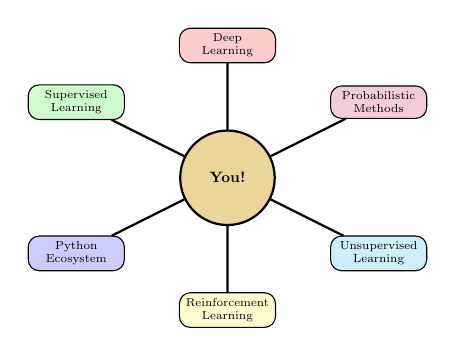
\begin{tikzpicture}[scale=0.6, transform shape]
    % Central node
    \node[circle, draw, thick, fill=hec-gold!40, minimum size=2cm, font=\small] (center) at (0,0) {\textbf{You!}};

    % Surrounding skills
    \node[rectangle, draw, fill=green!20, rounded corners, text width=1.8cm, text centered, font=\scriptsize] (sup) at (-3.2,1.6) {Supervised\\Learning};
    \node[rectangle, draw, fill=red!20, rounded corners, text width=1.8cm, text centered, font=\scriptsize] (dl) at (0,2.8) {Deep\\Learning};
    \node[rectangle, draw, fill=purple!20, rounded corners, text width=1.8cm, text centered, font=\scriptsize] (gp) at (3.2,1.6) {Probabilistic\\Methods};
    \node[rectangle, draw, fill=cyan!20, rounded corners, text width=1.8cm, text centered, font=\scriptsize] (unsup) at (3.2,-1.6) {Unsupervised\\Learning};
    \node[rectangle, draw, fill=yellow!20, rounded corners, text width=1.8cm, text centered, font=\scriptsize] (rl) at (0,-2.8) {Reinforcement\\Learning};
    \node[rectangle, draw, fill=blue!20, rounded corners, text width=1.8cm, text centered, font=\scriptsize] (tools) at (-3.2,-1.6) {Python\\Ecosystem};

    % Connections
    \draw[thick] (center) -- (sup);
    \draw[thick] (center) -- (dl);
    \draw[thick] (center) -- (gp);
    \draw[thick] (center) -- (unsup);
    \draw[thick] (center) -- (rl);
    \draw[thick] (center) -- (tools);
\end{tikzpicture}
\end{center}
\end{frame}

\begin{frame}{Thank You!}
\begin{columns}
\column{0.55\textwidth}
\begin{block}{Contact Information}
\textbf{Instructor}:\\
Simon Scheidegger\\
\href{mailto:simon.scheidegger@unil.ch}{simon.scheidegger@unil.ch}

\vspace{0.5em}
\textbf{Teaching Assistants}:\\
Maria Pia Lombardo\\
\href{mailto:mariapia.lombardo@unil.ch}{mariapia.lombardo@unil.ch}

\end{block}

\column{0.45\textwidth}
\begin{center}
\includegraphics[width=0.9\textwidth]{../../../fig/Ada_wrap-up.png}
\end{center}
\end{columns}

\vspace{0.5em}
\begin{center}
{\Large \textcolor{hec-blue}{Good luck with your capstone projects!}}
\end{center}
\end{frame}

\begin{frame}{Questions?}
\begin{center}
\vspace{2em}
{\Huge \textcolor{hec-blue}{Questions \& Discussion}}
\vspace{2em}

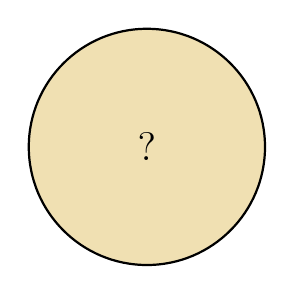
\begin{tikzpicture}
    \node[circle, draw, thick, fill=hec-gold!30, minimum size=3cm, font=\Large] {?};
\end{tikzpicture}
\end{center}
\end{frame}

% =============================================================================
% APPENDIX: ADDITIONAL REFERENCE SLIDES
% =============================================================================
\appendix

\begin{frame}{}
\begin{center}
{\Huge \textcolor{hec-blue}{Appendix}}\\[1em]
{\LARGE Reference Slides}
\end{center}
\end{frame}

\begin{frame}{Quick Reference: Loss Functions}
\begin{center}
\begin{tabular}{lll}
\toprule
\textbf{Task} & \textbf{Loss Function} & \textbf{Formula} \\
\midrule
Regression & MSE & $\frac{1}{N}\sum_i (y_i - \hat{y}_i)^2$ \\
Regression & MAE & $\frac{1}{N}\sum_i |y_i - \hat{y}_i|$ \\
Classification & Cross-entropy & $-\sum_i y_i \log(\hat{y}_i)$ \\
Classification & Hinge (SVM) & $\max(0, 1 - y_i \hat{y}_i)$ \\
\bottomrule
\end{tabular}
\end{center}

\vspace{1em}
\textbf{With Regularization}:
\begin{itemize}
    \item Ridge (L2): $\mathcal{L} + \lambda \|\w\|_2^2$
    \item Lasso (L1): $\mathcal{L} + \lambda \|\w\|_1$
    \item Elastic Net: $\mathcal{L} + \lambda_1 \|\w\|_1 + \lambda_2 \|\w\|_2^2$
\end{itemize}
\end{frame}

\begin{frame}{Quick Reference: Evaluation Metrics}
\begin{columns}
\column{0.5\textwidth}
\textbf{Regression}:
\begin{itemize}
    \item MSE: $\frac{1}{N}\sum(y - \hat{y})^2$
    \item RMSE: $\sqrt{\text{MSE}}$
    \item MAE: $\frac{1}{N}\sum|y - \hat{y}|$
    \item $R^2$: $1 - \frac{SS_{res}}{SS_{tot}}$
\end{itemize}

\column{0.5\textwidth}
\textbf{Classification}:
\begin{itemize}
    \item Accuracy: $\frac{TP + TN}{Total}$
    \item Precision: $\frac{TP}{TP + FP}$
    \item Recall: $\frac{TP}{TP + FN}$
    \item F1: $2 \cdot \frac{P \cdot R}{P + R}$
    \item AUC-ROC
\end{itemize}
\end{columns}

\vspace{1em}
\textbf{Clustering}:
\begin{itemize}
    \item Silhouette score: Measure cluster cohesion vs separation
    \item Davies-Bouldin index: Lower is better
    \item Adjusted Rand Index: Compare to ground truth
\end{itemize}
\end{frame}

\begin{frame}{Quick Reference: Key Equations}
\textbf{Linear Regression (closed form)}:
\[\hat{\w} = (\X^\top\X)^{-1}\X^\top\y\]

\textbf{Ridge Regression}:
\[\hat{\w} = (\X^\top\X + \lambda\mathbf{I})^{-1}\X^\top\y\]

\textbf{Logistic Regression}:
\[P(y=1|\x) = \sigma(\w^\top\x) = \frac{1}{1 + e^{-\w^\top\x}}\]

\textbf{Softmax (multi-class)}:
\[P(y=k|\x) = \frac{e^{\w_k^\top\x}}{\sum_j e^{\w_j^\top\x}}\]

\textbf{GP Posterior Mean}:
\[\mu_* = K_*^\top(K + \sigma^2I)^{-1}\y\]
\end{frame}

\begin{frame}{Week-by-Week Quick Reference}
{\small
\begin{tabular}{clll}
\toprule
\textbf{Week} & \textbf{Topic} & \textbf{Key Methods} & \textbf{Tools} \\
\midrule
1 & Intro to ML & -- & Nuvolos setup \\
2 & Holiday & -- & -- \\
3 & Python & -- & NumPy, Pandas, Jupyter \\
4 & Regression & Linear, Polynomial, Ridge, SGD & scikit-learn \\
5 & Gen AI & LLMs, Agents & (Guest lecture) \\
6 & Classification & kNN, Naive Bayes, Trees & scikit-learn \\
7 & Deep Learning & MLP, Backprop & TensorFlow \\
8 & DL Frameworks & RNN, LSTM & TF, PyTorch \\
9 & Applications & PINNs, DEQN, Recap & -- \\
10 & GPs & GP Regression, Kernels & GPFlow \\
11 & Dim. Reduction & PCA, Active Subspaces & scikit-learn \\
12 & Clustering & k-Means, GMM, DBSCAN & scikit-learn \\
13 & RL & Q-Learning, Portfolio & -- \\
14 & Wrap-up & Integration, Outlook & -- \\
\bottomrule
\end{tabular}
}
\end{frame}

\end{document}
